\section{System Architecture}
\label{sec:architecture}

CIM Wizard 2.0 comprises four layers: external datasources, semi data warehouse, operational database with multi-method calculators, and semantic VKG layer (Fig.~\ref{fig:architecture}).

\subsection{Design principles}

\begin{enumerate}[label=\textbf{D\arabic*.}, leftmargin=*]
  \item \textbf{Modular objectives} with O6 as integration proof.
  \item \textbf{Confidence over false precision}---expose uncertainty honestly.
  \item \textbf{Baseline compatibility}---Paper~1 priority-fallback mode remains available.
  \item \textbf{Validate every automation step}---SQL execution before OBDA commit.
\end{enumerate}

\subsection{Layered components}

\textbf{Semi data warehouse (O1).}
The \texttt{datalake/} service registers datasources as STAC Items with a \texttt{dl4r:} extension (source type, CRS, tags, ingest status).
Each ingest assigns a stable \texttt{datasource\_id} used in provenance records (O6).

\textbf{Operational database.}
PostgreSQL/PostGIS hosts \texttt{cim\_vector}, \texttt{cim\_census}, \texttt{cim\_network}, \texttt{cim\_raster}, 3DCityDB (\texttt{citydb}, \texttt{ng2\_*}), and TimescaleDB outputs.

\textbf{Feature computation (O6).}
The \texttt{PipelineExecutor} loads calculators from \texttt{configuration.json}.
In \texttt{baseline} mode, methods run in priority order until success (Paper~1).
In \texttt{all\_methods} mode, every configured method executes and emits a provenance record with optional confidence score.

\textbf{Semantic VKG (O2, O5).}
Ontop OBDA mappings (\texttt{cim\_citydb.obda}) virtualise relational data as RDF individuals typed with BOT, CityGML, SOSA, GeoSPARQL, and a project-specific \texttt{cim:} energy extension.
A multi-agent pipeline (O5) drafts new mapping blocks using fine-tuned text-to-SQL (O4) for \emph{source} SQL and ontology rules for \emph{target} RDF templates.

\begin{figure}[t]
  \centering
  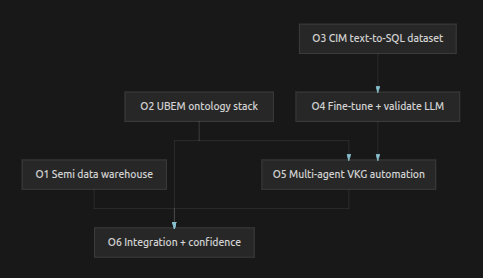
\includegraphics[width=0.92\linewidth]{figures/overall_schema}
  \caption{Overall CIM Wizard 2.0 schema: objectives O1--O6 and their dependencies. O3 feeds O4 (fine-tuning); O2 and O4 feed O5 (VKG automation); O1, O2, and O5 converge on O6 (integration and confidence).}
  \label{fig:architecture}
\end{figure}

Table~\ref{tab:repo} maps objectives to repository artefacts.

\begin{table}[t]
  \centering
  \caption{Repository mapping for objectives O1--O6.}
  \label{tab:repo}
  \small
  \begin{tabular}{cl}
    \toprule
    Obj. & Repository path \\
    \midrule
    O1 & \texttt{datalake/} \\
    O2 & \texttt{semantic/ontop/} \\
    O3 & \texttt{ai4db/} \\
    O4 & \texttt{txt2ssql/ftv2/}, \texttt{assist\_cim/} \\
    O5 & planned VKG agents + \texttt{semantic/SEMANTIC-plan.md} \\
    O6 & \texttt{cim\_wizard\_integrated\_2026/} \\
    \bottomrule
  \end{tabular}
\end{table}

\subsection{Comparison with Paper~1}

\begin{table}[t]
  \centering
  \caption{Paper~1 vs.\ Paper~2 architectural differences.}
  \label{tab:paper1vs2}
  \small
  \begin{tabular}{p{2.1cm}p{2.5cm}p{2.5cm}}
    \toprule
    Aspect & Paper~1 & Paper~2 \\
    \midrule
    Methods & Priority fallback & All methods \\
    Output & One value/feature & Matrix + provenance \\
    Data inputs & Ad hoc schemas & Warehouse registry \\
    Semantics & SQL/REST & UBEM ontology + VKG \\
    OBDA & Manual & LLM-assisted \\
    \bottomrule
  \end{tabular}
\end{table}
